\documentclass{beamer}
\usetheme{Singapore}
%\setbeamercolor{structure}{fg=red}
\usepackage{upgreek}
\usepackage{color}
%\def\magyarOptions{hyphenation=huhyphn}
%\usepackage{ae,aecompl}
%\usepackage[T1]{fontenc}
\usepackage[utf8]{inputenc}
%\usepackage[hungarian]{babel}
\usepackage{gensymb}
\usepackage{pgfplots}
\usepackage{pst-plot}
\usepackage{tikz}
\usepgfplotslibrary{external}
\tikzexternalize
\usepackage[version=3]{mhchem}

\normalfont
\title{Dekonvolúció a pásztázó elektrokémiai mikroszkópiában}
\subtitle{MKE Elektroanalitikai és Szenzorikai szakcsoport Szakmai Nap és Tisztújítás}
\author
{Kiss András\\
\hfill \\
}
\institute
{
  %\inst{1}%
  Általános és Fizikai Kémia Tanszék\\
  Pécsi Tudományegyetem\\
  \hfill \\

  \includegraphics[width=0.14\textwidth]{pte_logo.eps}\\
  Budapest, 2019. március 28.
}

\date[]

\begin{document}
\frame{\titlepage}  


\begin{frame}
	\centering
	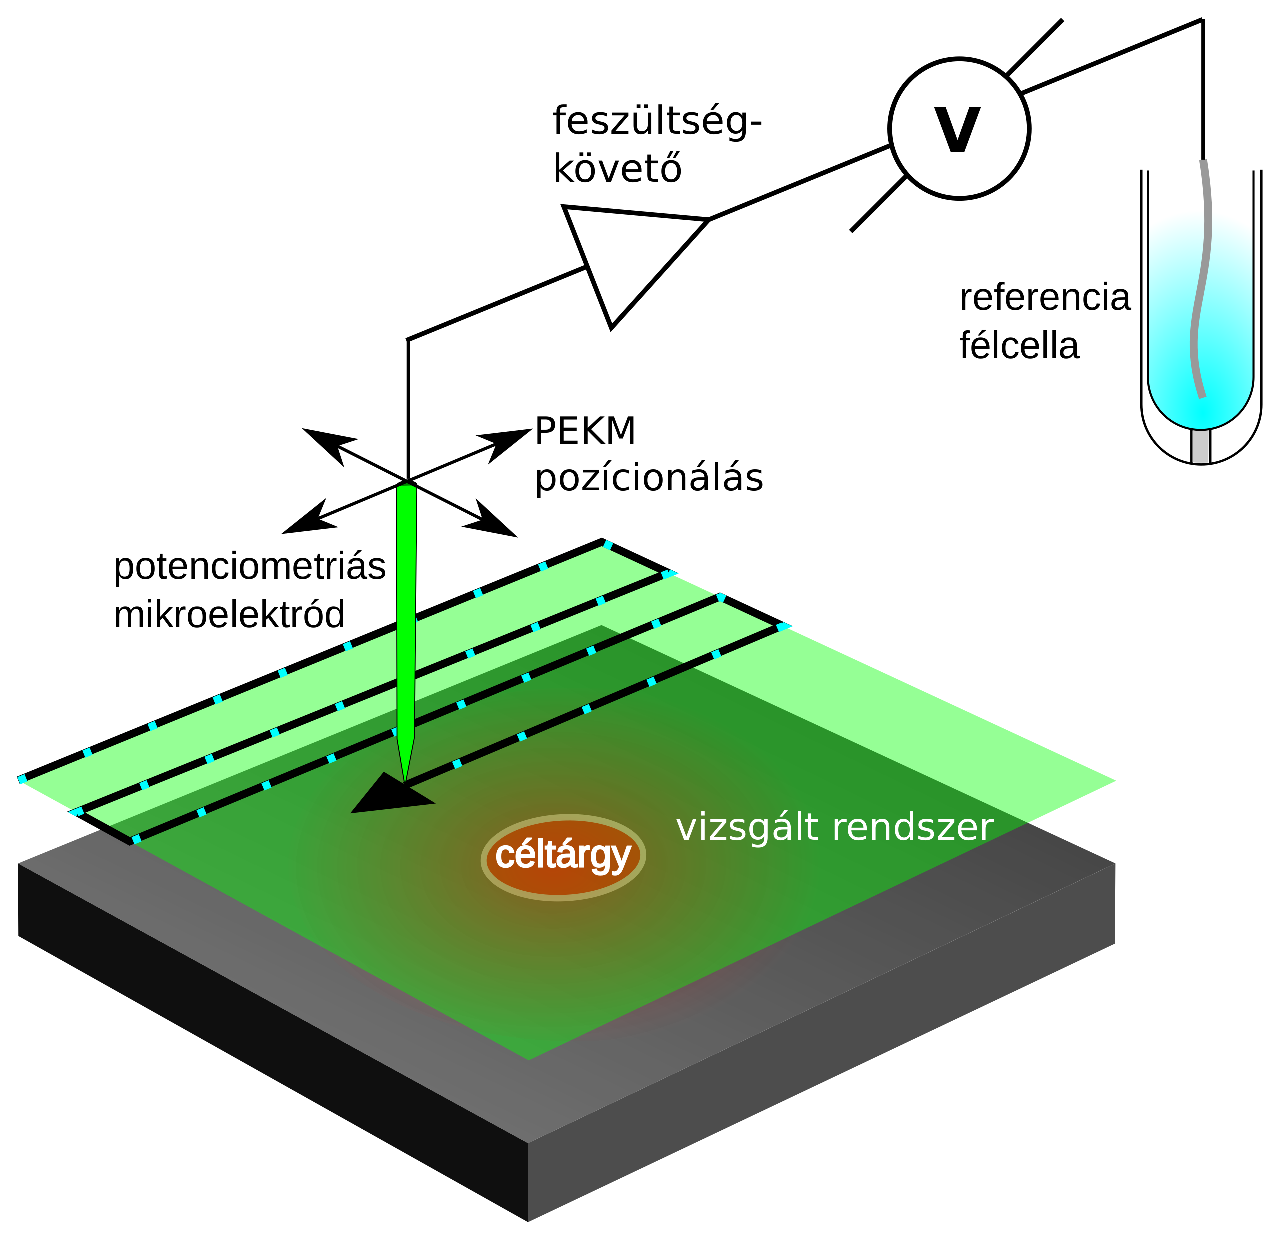
\includegraphics[width=0.6\textwidth]{secm.eps}
	\frametitle{Potenciometriás \underline{p}ásztázó \underline{e}lektro\underline{k}émiai \underline{m}ikroszkóp}
\end{frame}

\begin{frame}
\frametitle{Ion-szelektív mikropipetta}
\framesubtitle{PEKM mérőcsúcs}
\begin{columns}[T] % align columns
\begin{column}{.48\textwidth}

\centering
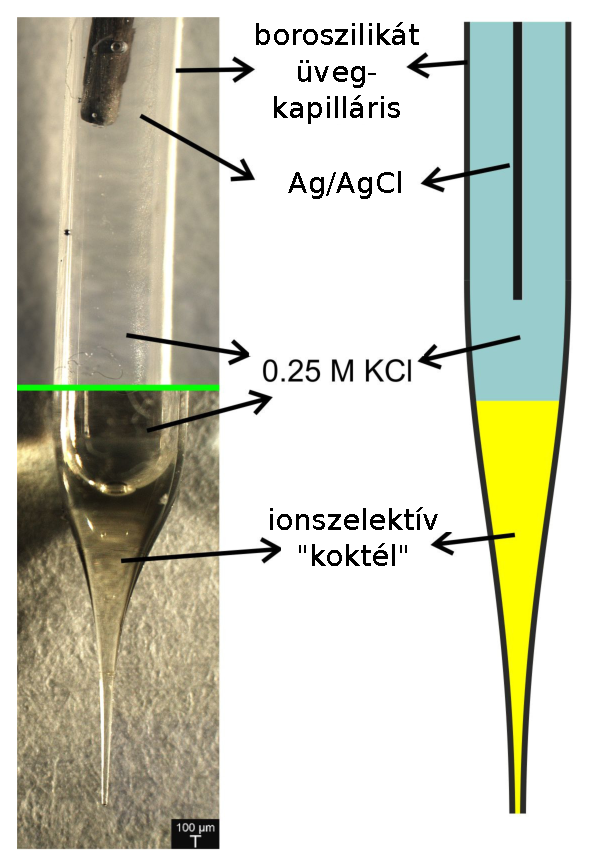
\includegraphics[width=0.9\textwidth]{liquid.eps}
\end{column}%
\hfill%
\begin{column}{.48\textwidth}
%\color{blue}\rule{\linewidth}{4pt}
\centering

\includegraphics[width=0.8\textwidth]{Valinomycin.eps}

Valinomicin
\vfill

\footnotesize
\begin{equation*}
        E=E^\theta + \frac{RT}{z_iF} \ln \left [ a_i + \sum_{j} \left ( k_{ij}a_j^{z_i/z_j} \right ) \right ]
        \end{equation*}
\normalsize
Nikolszkij--egyenlet
\end{column}%
\end{columns}
\end{frame}

\begin{frame}
\frametitle{Miért torzított a kép?}
\framesubtitle{Lehetséges okok}
\centering
\includegraphics[width=0.8\textwidth]{npp.eps}
\end{frame}

\begin{frame}
        \frametitle{Miért torzított a kép?}
        \framesubtitle{Az RC időállandó}
        \centering
        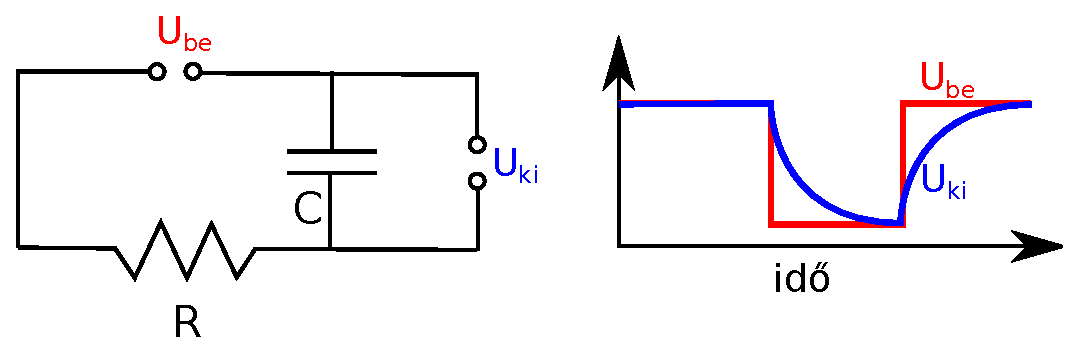
\includegraphics[width=1\textwidth]{RC.eps}
        \vfill
        A kondenzátor $\approx 63\%$-ra $(1-1/e)$ való töltéséhez szükséges idő. 
        \vfill
        $\tau = R \cdot C$

        $R = 5 $ G$\ohm$

        $C = 500 $ pF

        \textbf{\textcolor{white!100}{\colorbox{red!100}{$\tau = 2.5 $ s}}}

        %\includegraphics[width=0.6\textwidth, angle=-90]{meander_sim.eps}
\end{frame}

\begin{frame}
        \frametitle{A potenciometriás képalkotás torzítása}
        \framesubtitle{Vonalpásztázás esetén}
        \centering
        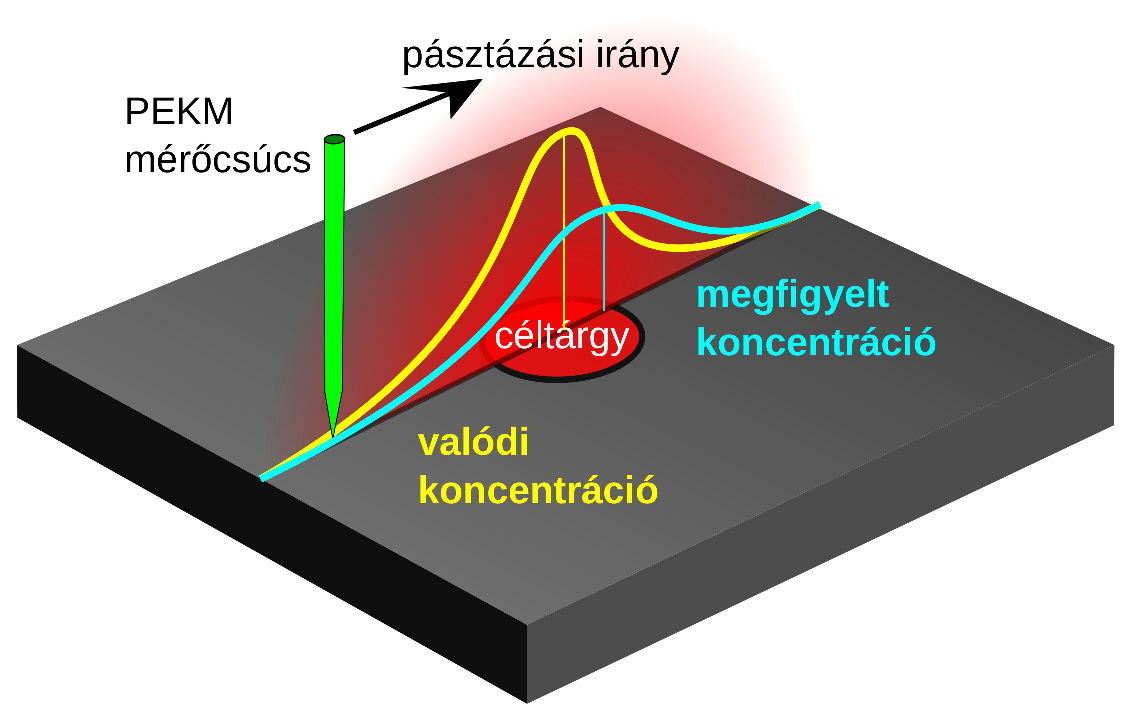
\includegraphics[width=0.8\textwidth]{distortion2.eps}
\end{frame}

\begin{frame}
        \frametitle{Miért fontos a pásztázás sebessége?}
        \framesubtitle{Példa: magnézium-ötvözet korróziója}
        \includegraphics[width=1\textwidth]{timelapse.eps}\\
\centering
Az AZ63 magnézium-alumínium ötvözet korróziója.
%Location of the anodic and cathodic spots change quickly. High-speed scanning is required to complete the scan before the studied system changes.
\end{frame}

\begin{frame}
\frametitle{A potenciometriás PEKM kompromisszum-diagramja}
\framesubtitle{Kompromisszum három kívánatos, de egymást kölcsönösen kizáró tulajdonság között}
\begin{center}
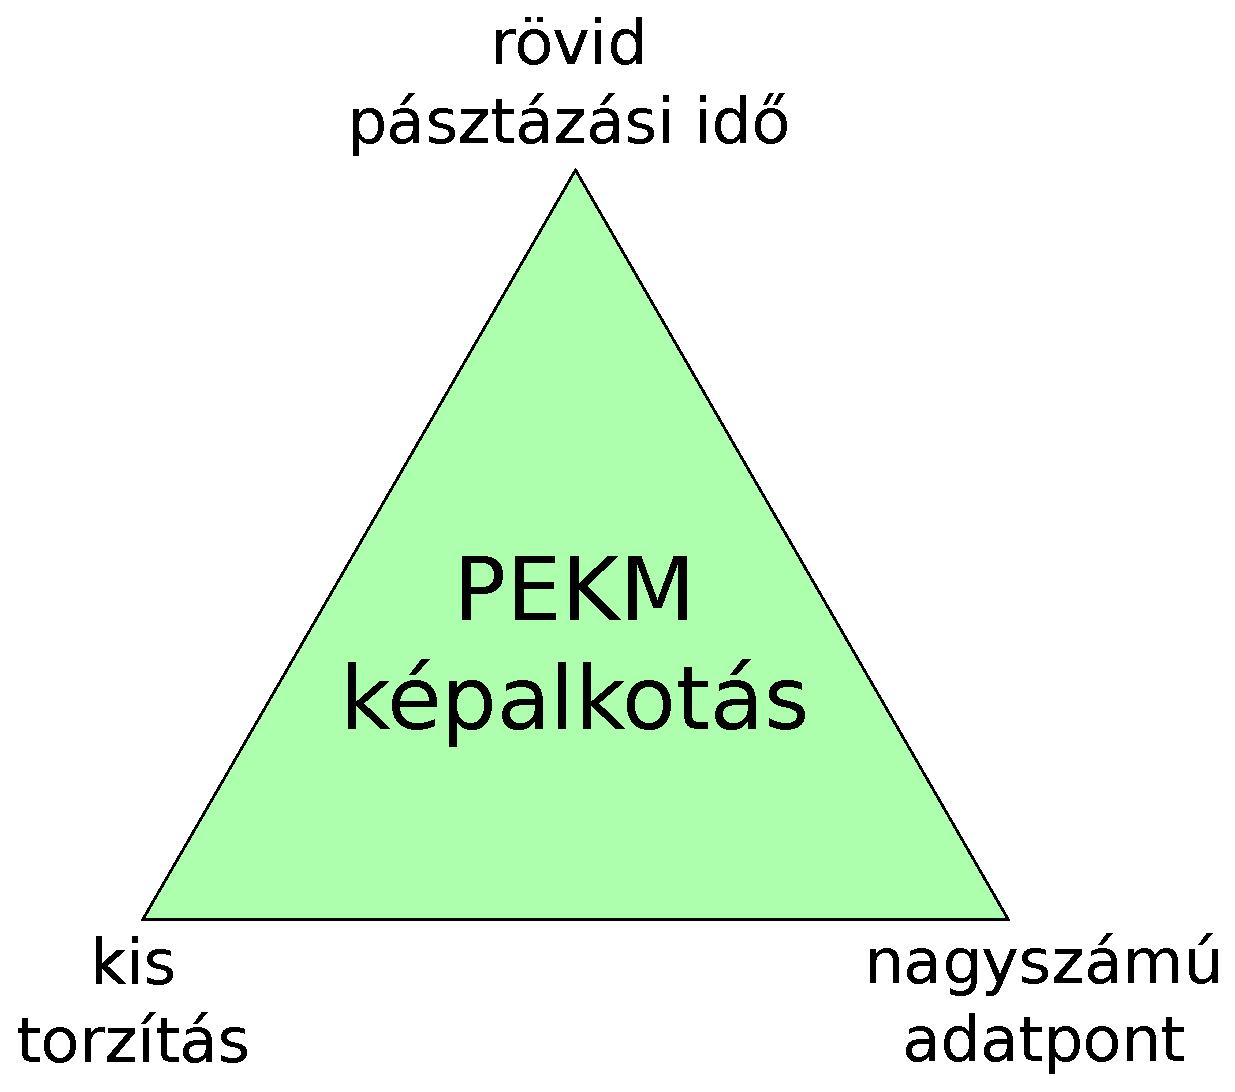
\includegraphics[width=0.5\textwidth]{trade-off.eps}
\end{center}
\end{frame}

\begin{frame}[plain]
\centering
1. megoldás: Szilárd-kontaktusú mikroelektródok használata.
\newline
\newline
2. megoldás: Pásztázási algoritmusok optimalizálása.
\newline
\newline
3. megoldás: Dekonvolúció.
\end{frame}

\begin{frame}
\frametitle{A torzítás konvolúciós függvénye}
\centering
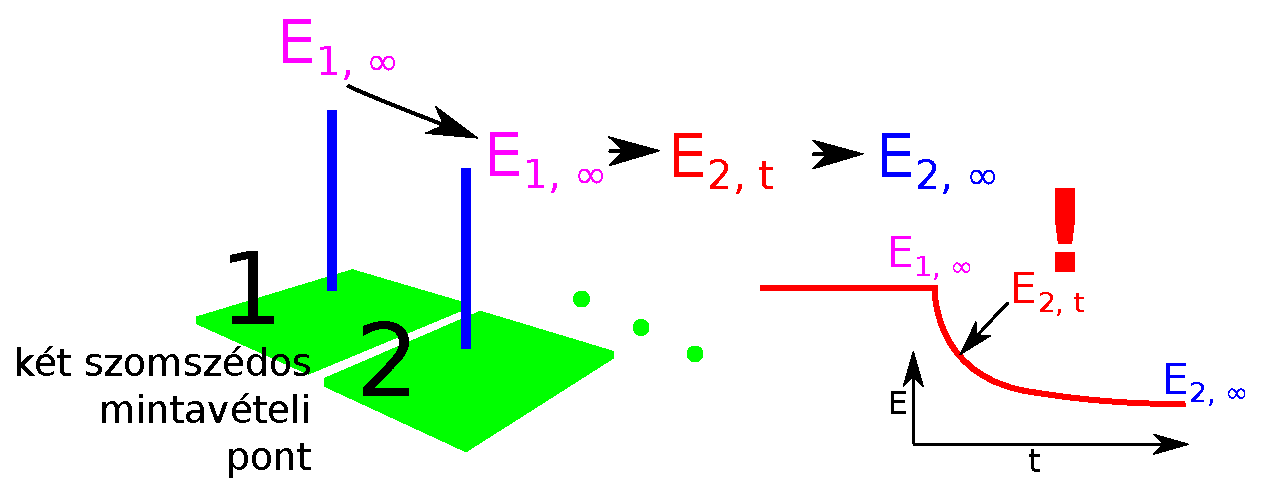
\includegraphics[width=1\textwidth]{t.eps}\\
\vfill
$E_{cell}(t) = E_{cell}(\infty) + [E_{cell}(0) - E_{cell}(\infty)]e^{-t/\tau}$\\
\vfill
%$E_{cell}(\infty)      = \frac {\displaystyle [E_{cell}(t) - E_{cell}(0)]e^{-t/RC}}    {\displaystyle 1 - e^{-t/RC}}$
\end{frame}

\begin{frame}
\frametitle{Konvolúció és dekonvolúció}
\centering
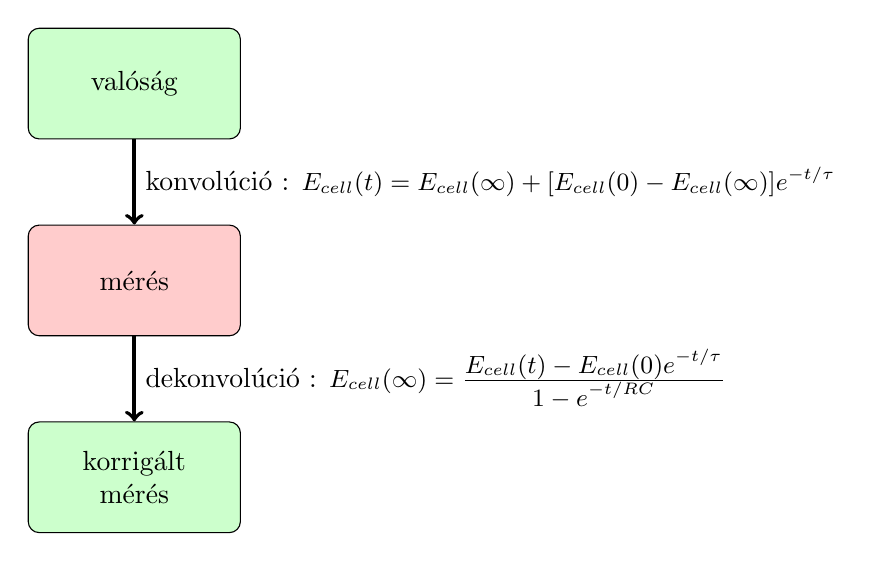
\begin{tikzpicture}[node distance = 2.5cm, auto]
\node [rectangle, draw, fill=green!20,text width=7em, text centered, rounded corners, minimum height=4em] (reality) {valóság};
\node [rectangle, below of=reality, draw, fill=red!20,text width=7em, text centered, rounded corners, minimum height=4em] (measurement) {mérés};
\node [rectangle, below of=measurement, draw, fill=green!20,text width=7em, text centered, rounded corners, minimum height=4em] (image) {korrigált\\ mérés};

\draw [line width=0.5mm, ->] (reality) -- (measurement) node [pos=.5, right] (TextNode) {konvolúció : \small $E_{cell}(t) = E_{cell}(\infty) + [E_{cell}(0) - E_{cell}(\infty)]e^{-t/\tau}$};
\draw [line width=0.5mm, ->] (measurement) -- (image) node [pos=.5, right] (TextNode) {dekonvolúció : \small $E_{cell}(\infty)      = \frac {\displaystyle E_{cell}(t) - E_{cell}(0)e^{-t/\tau}}    {\displaystyle 1 - e^{-t/RC}}$};
\end{tikzpicture}
\end{frame}

\begin{frame}
        \frametitle{Potenciometriás PEKM képek dekonvolúciója}
        \framesubtitle{pH-térképek az antimon mikroelektróddal}
\centering

\def\s{0.15}

\begin{columns}[T] % align columns

\begin{column}{.2\textwidth}
\begin{minipage}[c][0.75\textheight][c]{\linewidth}
\centering
%raw\\
%images
\end{minipage}
\end{column}%
\hfill%
\begin{column}{.2\textwidth}
\centering
\includegraphics[trim = 10mm 30mm 0mm 10mm, clip, width=0.8\textwidth, angle=-90]{13121313.eps}\\
\includegraphics[trim = 10mm 30mm 0mm 10mm, clip, width=0.8\textwidth, angle=-90]{13121314.eps}\\
\includegraphics[trim = 10mm 30mm 0mm 10mm, clip, width=0.8\textwidth, angle=-90]{13121315.eps}\\
\includegraphics[trim = 10mm 30mm 0mm 10mm, clip, width=0.8\textwidth, angle=-90]{13121316.eps}\\
\end{column}%
\begin{column}{.2\textwidth}
\begin{minipage}[c][0.7\textheight][c]{\linewidth}
\centering
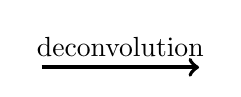
\begin{tikzpicture}
\draw [line width=0.5mm,->] (0,0) -- (2,0) node [pos=.5, above] (TextNode) {deconvolution};
\end{tikzpicture}
\end{minipage}
\end{column}%
\begin{column}{.2\textwidth}
\centering
\includegraphics[trim = 10mm 30mm 0mm 10mm, clip, width=0.8\textwidth, angle=-90]{13121313_deconvoluted.eps}\\
\includegraphics[trim = 10mm 30mm 0mm 10mm, clip, width=0.8\textwidth, angle=-90]{13121314_deconvoluted.eps}\\
\includegraphics[trim = 10mm 30mm 0mm 10mm, clip, width=0.8\textwidth, angle=-90]{13121315_deconvoluted.eps}\\
\includegraphics[trim = 10mm 30mm 0mm 10mm, clip, width=0.8\textwidth, angle=-90]{13121316_deconvoluted.eps}\\
\end{column}%
\begin{column}{.2\textwidth}
\begin{minipage}[c][0.75\textheight][c]{\linewidth}
\centering
%deconvoluted\\
%images
\end{minipage}
\end{column}%
\end{columns}
\end{frame}

\begin{frame}
\begin{center}
\frametitle{Potenciometriás PEKM képek dekonvolúciója}
\framesubtitle{Magnéziumion szelektív mikroelektróddal mért magnéziumion térképek}
\includegraphics[width=0.6\textwidth]{mg_2d.pdf}
\end{center}
\end{frame}

\begin{frame}
\frametitle{Gyakorlati példa: rozsdásodó szénacél}
\framesubtitle{pH-térkép, antimon mikroelektróddal mérve}
\begin{figure}
\centering
%top left bottom right
\includegraphics[trim = 10mm 30mm 0mm 10mm, clip, width=0.3\textwidth, angle=-90]{16012906.eps}\includegraphics[trim = 10mm 30mm 0mm 10mm, clip, width=0.3\textwidth, angle=-90]{16012906_deconvoluted.eps}

\includegraphics[width=0.24\textwidth]{cs_cut.jpg}

\end{figure}
\end{frame}


\begin{frame}
	\frametitle{Összefoglalás}
	\centering
\footnotesize
\begin{itemize}

\item A potenciometriás PEKM egy egyedülálló technika, mellyel valódi kémiai térképet nyerhetünk. Ez különösen előnyös korróziós vizsgálatokban.

\item Ezeket viszont gyorsan kell végezni, különben a vizsgált rendszer a mérés alatt jelentősen változik, és a mért adatpontoknak nemcsak a tér--, hanem az idő--koordinátái is eltérőek lesznek.

\item A pásztázási sebesség növelésével azonban nincs ideje a potenciometriás cellának az egyensúly elérésére az egyes mérési pontokon, ez torzítást okoz.

\item Kidolgoztam egy dekonvolúciós technikát a potenciometriás PEKM-hez, és példákon keresztül bemutattam, hogy ez jelentősen csökkenti a torzítást.

\item A technika segítségével a PEKM pásztázás sebesség legalább egy nagyságrenddel növelhető, és a nagy sebesség okozta torzítás a dekonvolúcióval korrigálható.

\end{itemize}
\end{frame}

\begin{frame}
	\centering
	Köszönöm a megtisztelő figyelmüket.
\end{frame}

\end{document}
